\chapter{Gerenciamento de Aplicações em Grade}
\label{cap:gerenciamento}

A idéia de computação em grade para processamento de aplicações em paralelo veio por consequência dos inúmeros avanços no desempenho de redes de computadores.

Atualmente o uso dessas redes tem aumentado exponencialmente. Muitas dessas redes são distribuídas de forma geograficamente separadas precisando de uma complexa infra-estrutura de software e hardware para gerenciá-las e conectá-las. Dentre as diversas soluções existentes a grade computacional (grid computing) possui características que viabiliza essa conexão.

O Open Grid Forum (OGF) uma comunidade fórum com milhares de indivíduos representando mais de 400 organizações em mais de 50 países criou e documentou \cite{M.2002} especificações técnicas e experiências de usuários. O OGF definiu grades computacionais como um ambiente persistente o qual habilita aplicações para integrar instrumentos, disponibilizar informações em locações difusas. Desde lá esta não é a única e precisa definição para o conceito de grades. Foster \cite{Kesselman2001} define um sistema em grade propondo um \emph{checklist} de três pontos.

\begin{enumerate}
	\item coordenar recursos os quais não são direcionados para um controle central.
	\item usar protocolos e interfaces padronizados, abertos para propósitos gerais.
	\item oferecer QoS (qualidade de serviço) não triviais tais como: autenticação, escalonamento de tarefas, disponibilidade.
\end{enumerate}

Uma definição formal do que um sistema em grade pode prover foi definido em \cite{Foster2002}. Focando na sua semântica, mostrando que grades não são apenas uma modificação de um sistema distribuído convencional. Podem apresentar recursos heterogênios como sensores e detectores e não apenas nós computacionais. Abaixo uma lista de aspectos que evidenciam uma grade computacional \cite{Cirne2002}:

\begin{itemize}
	\item heterogeneidade
	\item alta dispersão geográfica
	\item compartilhamento (não pode ser dedicado a uma única aplicação)
	\item múltiplos domínios administrativos (recursos de várias instituições)
	\item controle distribuído 
\end{itemize}

A grade deve estar preparada para lidar com todo o dinamismo e variabilidade, procurando obter a melhor performance possível adaptando-se ao cenário no momento.

\section{Gerenciamento de Recursos}

Devido à grande escala, ampla distribuição e existência de múltiplos domínios administrativos, a construção de um escalonador central de recursos para grades é praticamente inviável, até porque, convencer os administradores dos recursos que compõem a grade abrirem mão do controle dos seus recursos não é uma tarefa nada fácil. Escalonadores têm como características receber solicitações de vários usuários, arbitrando, portanto, entre os usuários, o uso dos recursos controlados.  

Casavant \cite{Thomas1996} considera escalonar como um problema de gerenciamento de recursos. Basicamente, escalonador é um mecanismo ou uma política usada para, eficientemente e efetivamente, gerenciar o acesso e uso de um determinado recurso. De acordo com o OGF's \cite{M.2002}, escalonamento é o processo de ordenar tarefas sobre os recursos computacionais e ordenar a comunicação entre as tarefas, assim sendo, ambas aplicações e sistemas devem ser escalonadas. 

O gerenciamento de recursos de um sistema centralizado possui informação completa e atualizada do estado (\emph{status}) dos recursos gerenciados. Este difere do sistema distribuído, o qual não tem conhecimento global de recursos dificultando assim, o gerenciamento. O ambiente em grade introduz cinco desafios para o problema de gerenciamento de recursos em ambientes distribuídos \cite{Karl1998}:

\begin{enumerate}
\item autonomia: os recursos são, tipicamente propriedades e operados por diferentes organizações em diferentes domínios administrativos;
\item heterogeneidade: diferentes lugares podem usar diferentes sistemas de gerenciamento de recursos (RMS);
\item extender as políticas: suporte no desenvolvimento de nova aplicação de mecanismos de gerência num domínio específico, sem necessitar de mudanças no código instalado nos domínios participantes;
\item co-alocação: algumas aplicações tem necessidades de recursos os quais só podem ser satisfeitos apenas usando recursos simultâneos com vários domínios;
\item controle online: RMSs precisam suportar negociações para adaptar necessidades de aplicações para recursos disponíveis.
\end{enumerate}

Sistemas computacionais, em muitos casos, falham ao tratar dois problemas \cite{Mangan2006}: 

\begin{itemize}
	\item gerenciamento e controle de um grande número de tarefas; 
	\item o balanceamento da carga da máquina de submissão e do tráfego da rede.
\end{itemize}

Uma distribuição dinâmica de dados e tarefas em uma hierarquia de gerenciadores poderia ajudar o gerenciamento de aplicações. O modelo GRAND baseado na submissão e controle particionados e hierárquicos foi detalhado em \cite{Mangan2006}. Uma explanação mais detalhada deste modelo será dada no próximo capítulo.

Grande parte das pesquisas sobre escalonamento de tarefas em grades seguem uma organização hierárquica ou centralizada tais como: Globus \cite{Foster1998}, Condor \cite{condor2007}, ISAM \cite{isam} e PBS \cite{Bayucan1998}.

Globus \cite{Globus}, um dos projetos mais referenciados na literatura, tem como principal software o Globus Toolkit (GT). Como o nome indica, o GT não é uma solução completa e sim um conjunto de serviços que podem ser combinados para a construção de um \emph{middleware} de grade. O Globus \cite{Foster1998} tem seu modelo de escalonamento centralizado. Não fornece suporte nativo as políticas de escalonamento mas permite que gerenciadores externos adicionem esta capacidade. O Globus (GT versão 3) oferece serviços de informação através de uma rede hierárquica chamada \emph{Metacomputing Directory Services} (MDS) \cite{Santos}. O gerenciamento de cada recurso é feito por uma instância do {\it Globus Resource Allocation Manager} (GRAM) \cite{Andrade2002}. GRAM é o responsável por instanciar, monitorar e reportar o estado das tarefas alocadas para o recurso. A GT4 \cite{Leon2006} disponibiliza tais serviços em uma arquitetura baseada em {\it Web Services} a {\it Open Grid Services Architecture} (OGSA) junto com {\it Web Services Resource Framework} (WSRF). A GT4 é focada na qualidade, robustez, facilidade de uso e documentação.

Outro projeto bastante importante é o Condor \cite{condor2007}, cujos trabalhos originais são voltados para redes de computadores, mas atualmente também contemplam {\it clusters} e grades. O Condor trabalha com a descoberta de recursos ociosos dentro de uma rede alocando esses recursos para execução das tarefas. Condor possui uma arquitetura de escalonamento centralizado, ou seja, uma máquina especial é responsável pelo escalonamento. Todas as máquinas podem submeter tarefas a máquina central que se responsabiliza de encontrar recursos disponíveis para execução da tarefa. Tanto o Condor quanto o Globus perdem pontos no quesito tolerância a falhas e escalabilidade devido ao fato de terem um controle centralizado onde um problema na máquina central comprometeria o sistema por inteiro. Além disso, para o Globus, são necessárias negociações com os donos de recursos além da necessidade do mapeamento dos clientes para usuários locais. O Condor permite interligar redes, desde que configurado manualmente para comunicar os escalonadores.

Já o projeto ISAM \cite{isam} possui uma arquitetura organizada na forma de células autônomas cooperativas. Sua proposta é fornecer uma infra-estrutura tanto para a construção quanto execução de aplicações pervasivas \cite {isam}. Concebida para habilitar as aplicações a obter informações do ambiente onde executam e se adaptam às alterações que ocorrem durante o transcurso da execução. O ISAM, diferente do Globus e do Condor, possui um modelo de escalonador de tarefas descentralizado ajudando o sistema a alcançar um bom nível de tolerância a falhas e escalabilidade.

Um dos gerenciadores que podem ser integrados com o Globus é o PBS \cite{Bayucan1998}. O PBS é um RMS que tem por propósito prover controle adicionais sobre a execução de tarefas em batch. O sistema permite um domínio definir e implementar políticas tais como os tipos de recursos e como esses recursos podem ser usados por diferentes tarefas.

\section{Portable Batch System - PBS}
%\label{cap:pbs}

Desenvolvido para fornecer processamento em lote, ao contrário de colocar um processo em segundo plano, o processamento em lote do PBS abrange o escalonamento de múltiplas tarefas conforme as políticas do RMS. Cada tarefa pode conter inúmeros processos. Essas tarefas podem ser direcionadas para rotear processos através de nós em uma rede. É possível a reserva de recursos para determinada tarefa antes do início da sua execução \cite{Bayucan1998a}.

\section{PBS - Cliente}

Comandos devem estar de acordo com a especificação POSIX.15. É possível especificar mais de uma operação na linha de comando onde essas serão interpretadas uma de cada vez. A geração de um erro de operando em determinado servidor será colocado na saída de erro padrão. O comando continua executando demais operandos. Sendo que o recebimento de qualquer erro por qualquer operando, resultará em um \emph{status} final maior que zero.

\section{PBS - Servidor}

O servidor principal tem como foco principal a comunicação dos clientes e gerenciar as tarefas. O servidor é o coração do sistema e suas principais responsabilidades são \cite{Bayucan1998a}:

\begin{itemize}
	\item possuir e controlar tarefas em lotes.
	\item possuir e controlar filas.
	\item recuperar estado de tarefas e filas.
	\item executar serviços em nome de clientes baseado em um serviço de requisição de lote.
	\item executar serviços adiados em nome de tarefas baseadas em eventos externos.
	\item iniciar seleção de tarefas para execução baseado em um grupo local definido de políticas de regras.
	\item estabelecer recursos reservados e usar limites para tarefas iniciadas no local de execução.
	\item colocar uma tarefa de lote em execução e monitorar seu progresso.
	\item executar o processamento e a limpeza de tarefas.
\end{itemize}

\section{Processo de Escalonamento}

O processo de escalonamento se caracteriza por uma escolha que elege qual tarefa será executada. Para isto, esta tarefa deve constar em uma fila de execução.

O PBS fornece um programa separado como um processo de seleção que maximiza a flexibilidade na implementação das políticas locais. O escalonador comunica-se com o servidor via um \emph{socket} IPC. Desta forma é possível possuir escalonador e servidor em diferentes nós.

Para cumprir seu papel de gerenciador de recursos, o escalonador se comunica com outro processo chamado \emph{Machine Oriented Mineserver} (MOM). Assim é possível recuperar informações sobre a carga do sistema do nó. Nestas informações podem conter detalhes do uso de memória, carga de CPU, entre outras. Esta relação entre PBS, o escalonador e o MOM é demostrado na figura~\ref{fig:Pbs_MOM} \cite{Bayucan1998}.

\begin{center}
	\begin{enumerate}
		\item Evento aviso o servidor para iniciar um ciclo de escalonamento.
		\item Servidor envia comando de escalonamento para Escalonador.
		\item Escalonador requisita informação de recursos do MOM.
		\item MOM retorna informações solicitadas.
		\item Escalonador requisita informações do servidor.
		\item Servidor envia informações de \emph{status} da tarefa para o escalonador. Escalonador realiza política para executar a tarefa.
		\item Escalonador envia solicitação de execução para o servidor.
		\item Servidor envia tarefa para o MOM executar.
	\end{enumerate}
\end{center}

\begin{figure}[htb]
\begin{center}
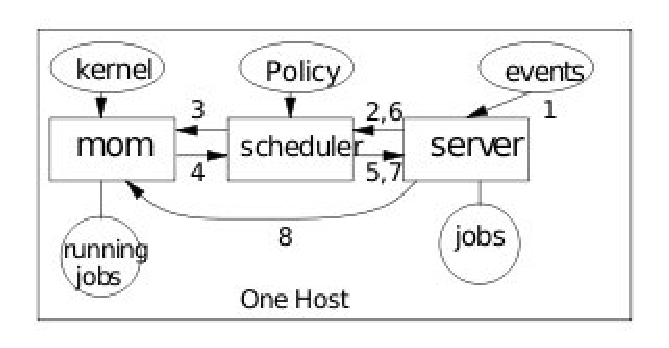
\includegraphics[scale=0.9]{./img/PbsMom.eps}
\caption{Escalonamento em um nó}
\label{fig:Pbs_MOM}
Fonte: \cite{Bayucan1998}
\end{center}
\end{figure}

Um ponto negativo no PBS é o fato deste ter um servidor centralizando, onde uma pane neste nó, afetaria o sistema por inteiro.

Para acesso as funcionalidades que o PBS oferece são fornecidas duas maneiras, um conjunto de \emph{scripts} de linha de comando e uma biblioteca de programação. A biblioteca escrita na linguagem C denominada \emph{Batch Interface Library} (IFL).

O próximo capítulo faz uma análise sobre o modelo GRAND, suas características bem como o protótipo AppMan desenvolvido nos padrões do modelo GRAND.
\chapter{Modelo GRAND}
\label{cap:grand}

No modelo GRAND são tratados três aspectos do gerenciamento de dados: transferência automática dos dados de entrada para o local onde o arquivo será necessário; o envio de resultados é controlado evitando congestionamento da rede; priorização de localidade no disparo de tarefas para não haver transferências desnecessárias de dados degradando o desempenho. Através de uma hierarquia de gerenciadores (Figura 1) é feito o disparo e controle das aplicações. o \emph{Application Manager} (AP) recebe uma submissão de aplicação através de um usuário, os APs mandam os \emph{Submission Managers} (SM) descrições de tarefas assim, sob demanda, são instanciados os \emph{Task Managers} (TM) para controlar a submissão de tarefas a escalonadores de domínios específicos da grade, esses escalonadores recebem requisições dos TMs fazendo a execução das tarefas propriamente ditas.

Pelo fato de que, na atualidade, ambientes grades envolvem principalmente instituições de ensino em aplicações usualmente classificadas como aplicações científicas, o escopo do GRAND é limitado as seguintes itens. 

\begin{enumerate}
    \item heterogeneidade, lembrando que isto afeta diretamente a política de escalonamento por necessitar de saber as características distintas de hardware e software; 
    \item grande número de submissão de tarefas, referindo-se a aplicações que geram centenas ou milhares de processos; 
    \item ausência de comunicação por troca de mensagens, pelo fato da necessidade de inúmeros aspectos nas fases de agrupamento e mapeamento serem considerados; 
    \item interdependência de tarefas, devido ao compartilhamento de arquivos; 
    \item manipulação de grande número de arquivos pelas tarefas; 
    \item o uso de arquivos grandes, através de técnicas como \emph{staging} e \emph{caching}, minimizando a perda de desempenho em função da latência de transmissão; 
    \item segurança, assume-se que exista uma conexão segura entre os nós da grade; 
    \item descoberta dinâmica de recursos; 
    \item gerenciador de recursos local em cada nó; 
    \item uma tarefa é executada em um RMS até sua finalização;
\end{enumerate}

\begin{figure}[htb]
\begin{center}
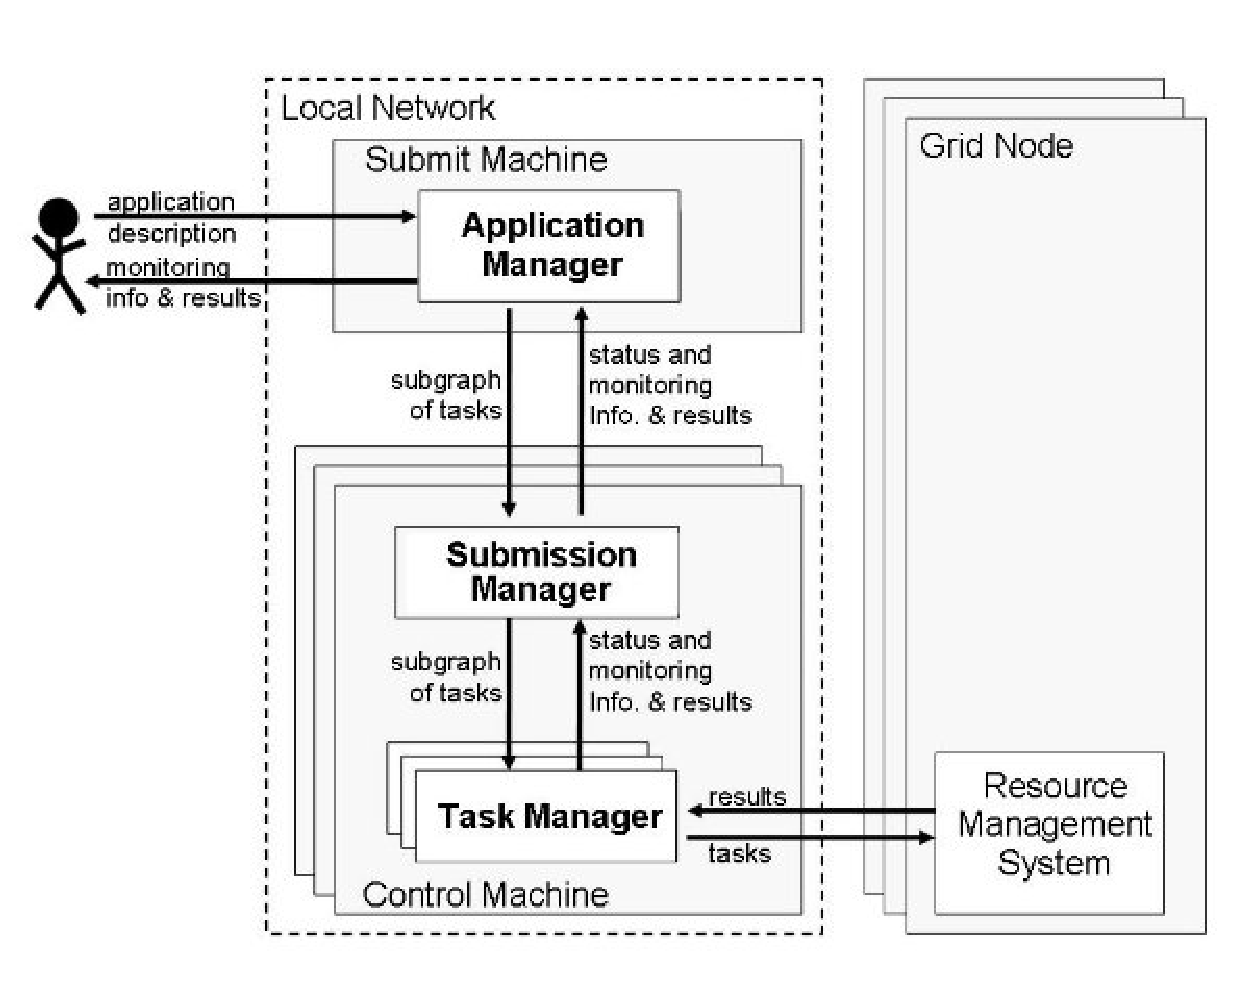
\includegraphics[scale=0.7]{./img/grand.eps}
\caption{Principais componentes do modelo hierárquico de gerenciamento de tarefas}
\label{fig:Modelo_Grand}
\end{center}
\end{figure}

\section{Característica das Aplicações}

Baseando-se em aplicações típicas para ambientes de grades, comunicando-se via troca de arquivo, conhecimento do número de processo a serem criados e sem troca de mensagens, é proposta a seguinte taxonomia de aplicações \emph{ver as bibliografias que consta na página 23 da tese da kayser}

\begin{itemize}
	\item tarefas independentes \emph{\textbf{independent tasks}} ou seja, as tarefas não possuem dependência entre si. Muitas vezes chamado de \emph{bag-of-tasks}.
	\item tarefas fracamente acopladas \emph{\textbf{loosely-coupled tasks}} tarefas com poucos pontos de compartilhamentos, aplicações dividas em fases ou sequência.
	\item tarefas fortemente acopladas \emph{\textbf{tightly-coupled tasks}} grafos complexos, aplicações em lógica com restrições.
\end{itemize}

\begin{figure}[htb]
\begin{center}
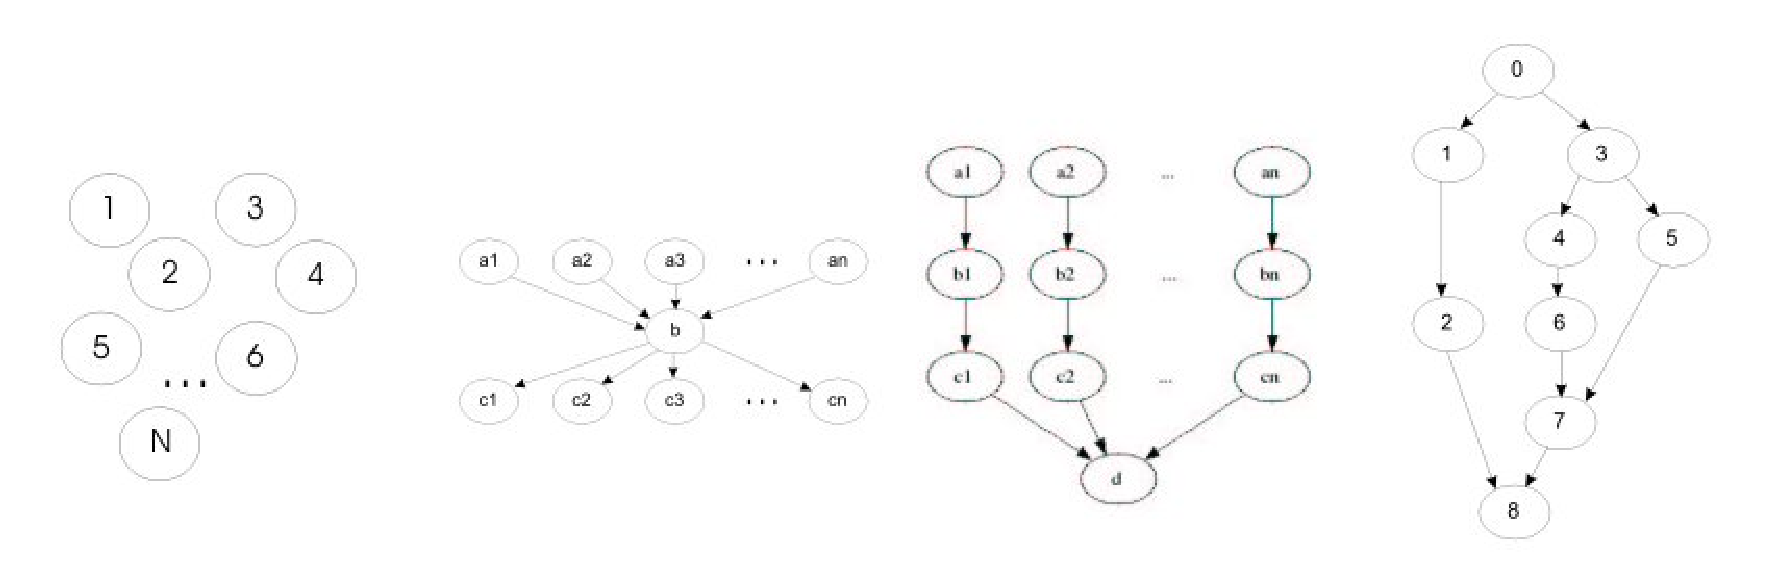
\includegraphics[scale=0.5]{./img/TaxonomiaAplicacoes.eps}
\caption{Categorias de aplicações de grade: (a) \emph{independent tasks}, (b) \emph{loosely-coupled task(phase)}, (c) \emph{loosely-coupled tasks (pipeline)} e (d) \emph{tightly-coupled tasks}}
\label{fig:Taxonomia_Aplicacoes}
\end{center}
\end{figure}

\section{Gerenciamento de Dados}

Ainda há muito o que ser feito nesta questão, até então o tratamento dos dados é resolvido através de soluções distintas. A preocupação principal de vários trabalhos \emph{CITAR GLOBUS E GRIDFTP} é com dados em forma de arquivos.

No GRAND, o gerenciamento de arquivos é apenas com \emph{stage in} e \emph{stage out}, ou seja, enviar os dados para o local de processamento e retorno de resultados. 


\section{Particionamento}

\section{Modelo de Gerenciamento}
